\subsection{Подход Клайнберга}

    Следующий подход предложил Американский математик Джон Клайнберг. \cite{Kleinberg, Kleinberg2}
%     Следующий подход предложил Американский математик Джон Клайнберг. Перед началом разбора,
% мне бы хотелось сделать некоторую поправку. Джон Клайнберг в своих статьях нигде не 
% упоминает о коэффиценте класстеризации. Вместо этого он говорит только о наличии длинных
% и коротких рёбер. Это немного расширяет класс "Тесных" графов, однако идейно 
% ничего не меняет.

    Изучим заново граф, который изображён на Рис. \ref{lattice}. Он состоит только из
коротких связей, а значит, тесным графом не является. Есть разные способы решить эту проблему,
давайте рассмотрим предложение Джона Клайнберга, так как его метод формирования длинных
рёбер очень естественно вписывается в окружающий нас мир. Идея проста: чем человек дальше от меня, тем меньше
вероятность нашего знакомства. Формально его идею можно записать так, 
Графу даются 2 параметра p, k:
\begin{itemize}
    \item p - радиус. Все вершины, расстояние между которыми меньше или равно p, мы соединяем ребром и 
    и называем короткой связью
    \item k - кол-во длинных связей. После добавления коротких связей, останется только пройтись по всевозможным 
    парам вершин и расставить рёбра в зависимости от следующего распределения:
\end{itemize}

\begin{equation} \label{edges_distribution}
    P(u \rightarrow v) = \frac{1}{d(u, v)^r}\frac{1}{C}, \text{ где } C = \sum_{u \neq z \in V}\frac{1}{d(u, z)^r}
\end{equation}

Во время своего исследования, он пришёл к выводу, что наилучший результат достигается при 
r = d, где d - размерность пространства. Причём кол-во длинных рёбер должно быть 
примерно равно $q = \log{n}$.

\subsubsection{Построение структуры}
Алгоритм построения представлен в виде блок схемы. Хочу заметить, что асимптотическая
сложность построения данной стркутуры очень большая ($O(n^2)$), что делает её мало где применимым.
Однако граф Клайнберга - является больше идеей. Её можно внедрять в другие структуры для 
их модификации 

\begin{figure}[H]
    \centering
    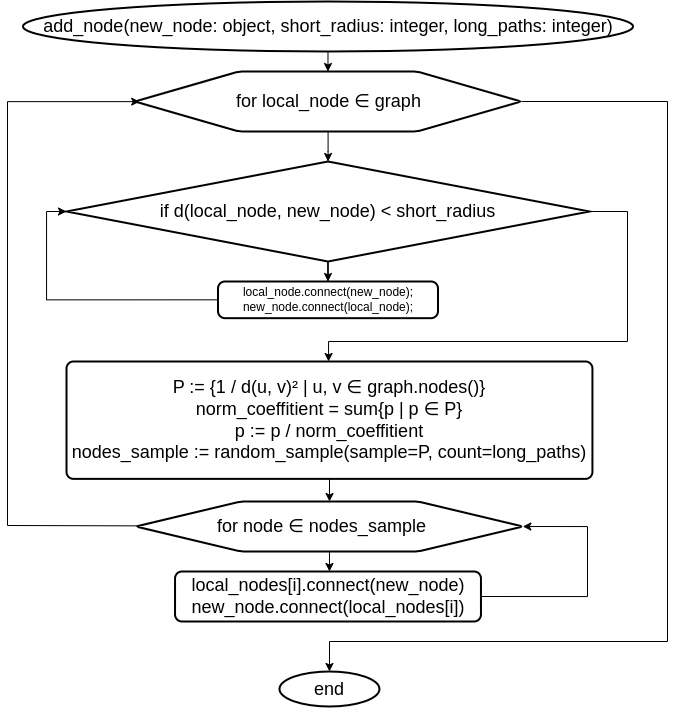
\includegraphics[scale=0.6]{./pictures/Kleinberg_add_node.png}
    \caption{Блок схема построение графа по методу Джона Клайнберга} \label{Kleinberg_graph_block_scheme}
\end{figure}



